\documentclass{article}
\usepackage[T1]{fontenc}
\usepackage[letterpaper, margin=2cm]{geometry}
\usepackage{amsmath, amsthm, amssymb}
\usepackage{mathtools}
\usepackage{epigraph}
\usepackage{graphicx}
\usepackage[inline]{enumitem}
\usepackage[noend]{algpseudocode}
\usepackage{float} % for exact placement of floats
\usepackage[dvipsnames]{xcolor} % for color names, must be loaded before tikz
\usepackage{tikz}
\usepackage[framemethod=tikz]{mdframed}
\usepackage{environ, varwidth}
\usepackage{hyperref}
\usepackage{bm}
\usepackage[normalem]{ulem}
\usepackage[outline]{contour}
\usepackage{newtxtext, newtxmath}
\usepackage{pifont} % for xmark and cmark
\usepackage{subdepth} % prevents superscripts from affecting subscript positioning

\hypersetup{
    colorlinks,
    linkcolor={red!50!black},
    citecolor={blue!50!black},
    urlcolor={blue!80!black}
}

% makes math in headlines bold
%\makeatletter
%\g@addto@macro\bfseries{\boldmath}
%\makeatother
\contourlength{1pt}
\renewcommand{\ULdepth}{2pt}
\renewcommand{\ULthickness}{0.5pt}
\renewcommand{\descriptionlabel}[1]{%
  \hspace{\labelsep}\normalfont\uline{\phantom{#1}}\llap{\contour{white}{#1}}\hfill% 
}

% lemmas/theorems/definitions
\newtheoremstyle{customstyle}%            % Name
  {}%                                     % Space above
  {}%                                     % Space below
  {}%                                     % Body font
  {}%                                     % Indent amount
  {\bfseries}%                            % Theorem head font
  {.}%                                    % Punctuation after theorem head
  { }%                                    % Space after theorem head, ' ', or \newline
  {\thmname{#1}\thmnumber{ #2}\thmnote{ (#3)}}%
\theoremstyle{customstyle}

% mdframed's skipbelow is buggy and needs a patch
\usepackage{xpatch}
\makeatletter
\xpatchcmd{\endmdframed}
  {\aftergroup\endmdf@trivlist\color@endgroup}
  {\endmdf@trivlist\color@endgroup\@doendpe}
  {}{}
\makeatother

\newmdtheoremenv[innertopmargin=-2pt, skipabove=5pt, skipbelow=0pt, linewidth=2pt, linecolor=Green, backgroundcolor=Green!10, bottomline=false, leftline=false, rightline=false]{theorem}{Theorem}
\newmdtheoremenv[innertopmargin=-2pt, skipabove=5pt, skipbelow=0pt, linewidth=2pt, linecolor=Green, backgroundcolor=Green!10, bottomline=false, leftline=false, rightline=false]{lemma}{Lemma}
\newmdtheoremenv[innertopmargin=-2pt, skipabove=5pt, skipbelow=0pt, linewidth=2pt, linecolor=Green, backgroundcolor=Green!10, bottomline=false, leftline=false, rightline=false]{corollary}{Corollary}
\newmdtheoremenv[innertopmargin=-2pt, skipabove=5pt, skipbelow=0pt, linewidth=2pt, linecolor=Yellow, backgroundcolor=Yellow!10, bottomline=false, leftline=false, rightline=false]{definition}{Definition}

\newenvironment{prf}{\begin{mdframed}[skipabove=5pt, backgroundcolor=Gray!10, topline=false, bottomline=false, leftline=false, rightline=false]\begin{proof}}{\end{proof}\end{mdframed}}

\setlength{\parindent}{0.25cm}
\setlength{\epigraphwidth}{\textwidth}

% pseudo code
% makes the pseudo code a little less verbose
\renewcommand\algorithmicfunction{}
\renewcommand\algorithmicthen{}
\renewcommand\algorithmicdo{}

\newenvironment{algo}{\begin{samepage}\medskip\hrule\begin{algorithmic}}{\end{algorithmic}\hrule\medskip\end{samepage}}

% quote and unquote for formal strings
\newcommand{\qu}[1]{\mathsf{#1}}
\newcommand{\uq}[1]{\text{$#1$}}

% Formulas
\newcommand{\textscsf}[1]{\textsf{\textsc{#1}}}
\DeclareMathOperator{\Con}{\textscsf{Con}}
\DeclareMathOperator{\Pvb}{\textscsf{Pvb}}
\DeclareMathOperator{\Pvbp}{\textscsf{Pvb\textquotesingle}}
\DeclareMathOperator{\Chk}{\textscsf{Ck}}

% Functions
\newcommand{\eq}{\mathrel{\resizebox{1.15\height}{1.15\height}{=}}}
\DeclareMathOperator{\pc}{\mathit{pc}}
\DeclareMathOperator*{\bast}{\scalebox{1.15}{$\bm{\ast}$}}
\DeclareMathOperator*{\argmin}{arg\,min}

% Delimiters
\newcommand{\rep}[1]{\text{\guilsinglleft$#1$\guilsinglright}}

% Constants
\newcommand{\qutick}{\textbf{\textquotesingle}}
\newcommand{\T}{\textbf{\textsf{T}}}
\newcommand{\Q}{\textbf{\textsf{Q}}}
\newcommand{\PA}{\textbf{\textsf{PA}}}
\newcommand{\cmark}{\text{\small \ding{51}}}
\newcommand{\xmark}{\text{\small \ding{55}}}
\newcommand{\imp}{\parbox{0.125cm}{\tikz{\draw[->](0,0)--(0.125cm,0);}}}

% Numeral corner quotes
\newbox\numBoxA
\newdimen\numCornerHgt
\setbox\numBoxA=\hbox{\footnotesize $\ulcorner$}
\global\numCornerHgt=\ht\numBoxA
\newdimen\numArgHgt
\def\num #1{%
\setbox\numBoxA=\hbox{$#1$}%
\numArgHgt=\ht\numBoxA%
\ifnum     \numArgHgt<\numCornerHgt \numArgHgt=0pt%
\else \advance \numArgHgt by -\numCornerHgt%
\fi \raise\numArgHgt\hbox{\footnotesize $\ulcorner$} \box\numBoxA %
\raise\numArgHgt\hbox{\footnotesize $\urcorner$}}

\newcommand{\numrep}[1]{\num{\hspace{-3.33pt}\rep{#1}\hspace{-3.33pt}}}


\begin{document}

\title{\vspace{-1cm}What If Turing Had Preceded Gödel?}
\author{Sebastian Oberhoff\\{\small oberhoff.sebastian@gmail.com}}
\date{\today}

\maketitle

\begin{abstract}
  The main message of the following pages is that mathematical logic---centered around the incompleteness theorems---is first and foremost an investigation of \emph{computation}, not arithmetic. More concretely, we're going to hone in on one key fact: Peano Arithmetic can represent any computable function. It has achieved Turing completeness. Armed with this knowledge we will show the following.
  \begin{itemize}
    \item We'll derive the Diagonal Lemma and First Incompleteness Theorem using significantly simplified proofs.
    \item Using self-referential trickery we'll be able to avoid much of the technical morass surrounding the Second Incompleteness Theorem, arriving at two versions: one which uses the HBL-derivability conditions, and one which doesn't.
    \item Drawing on analogy between the First Incompleteness Theorem and the Halting Problem produces an equivalent of the Nondeterministic Time Hierarchy Theorem from the field of computational complexity.
    \item Finally, we'll generalize the First Incompleteness Theorem in the presence of oracles.
  \end{itemize}
\end{abstract}

\epigraph{In March of 1977, I met the great AI pioneer Marvin Minsky for the first time. It was an unforgettable experience. One of the most memorable remarks he made to me was this one: ``Gödel should just have thought up Lisp; it would have made the proof of his theorem much easier.'' I knew exactly what Minksy meant by that, I could see a grain of truth in it, and moreover I knew it had been made with tongue semi in cheek.}{\textit{Douglas Hofstadter}}

\begin{center}
  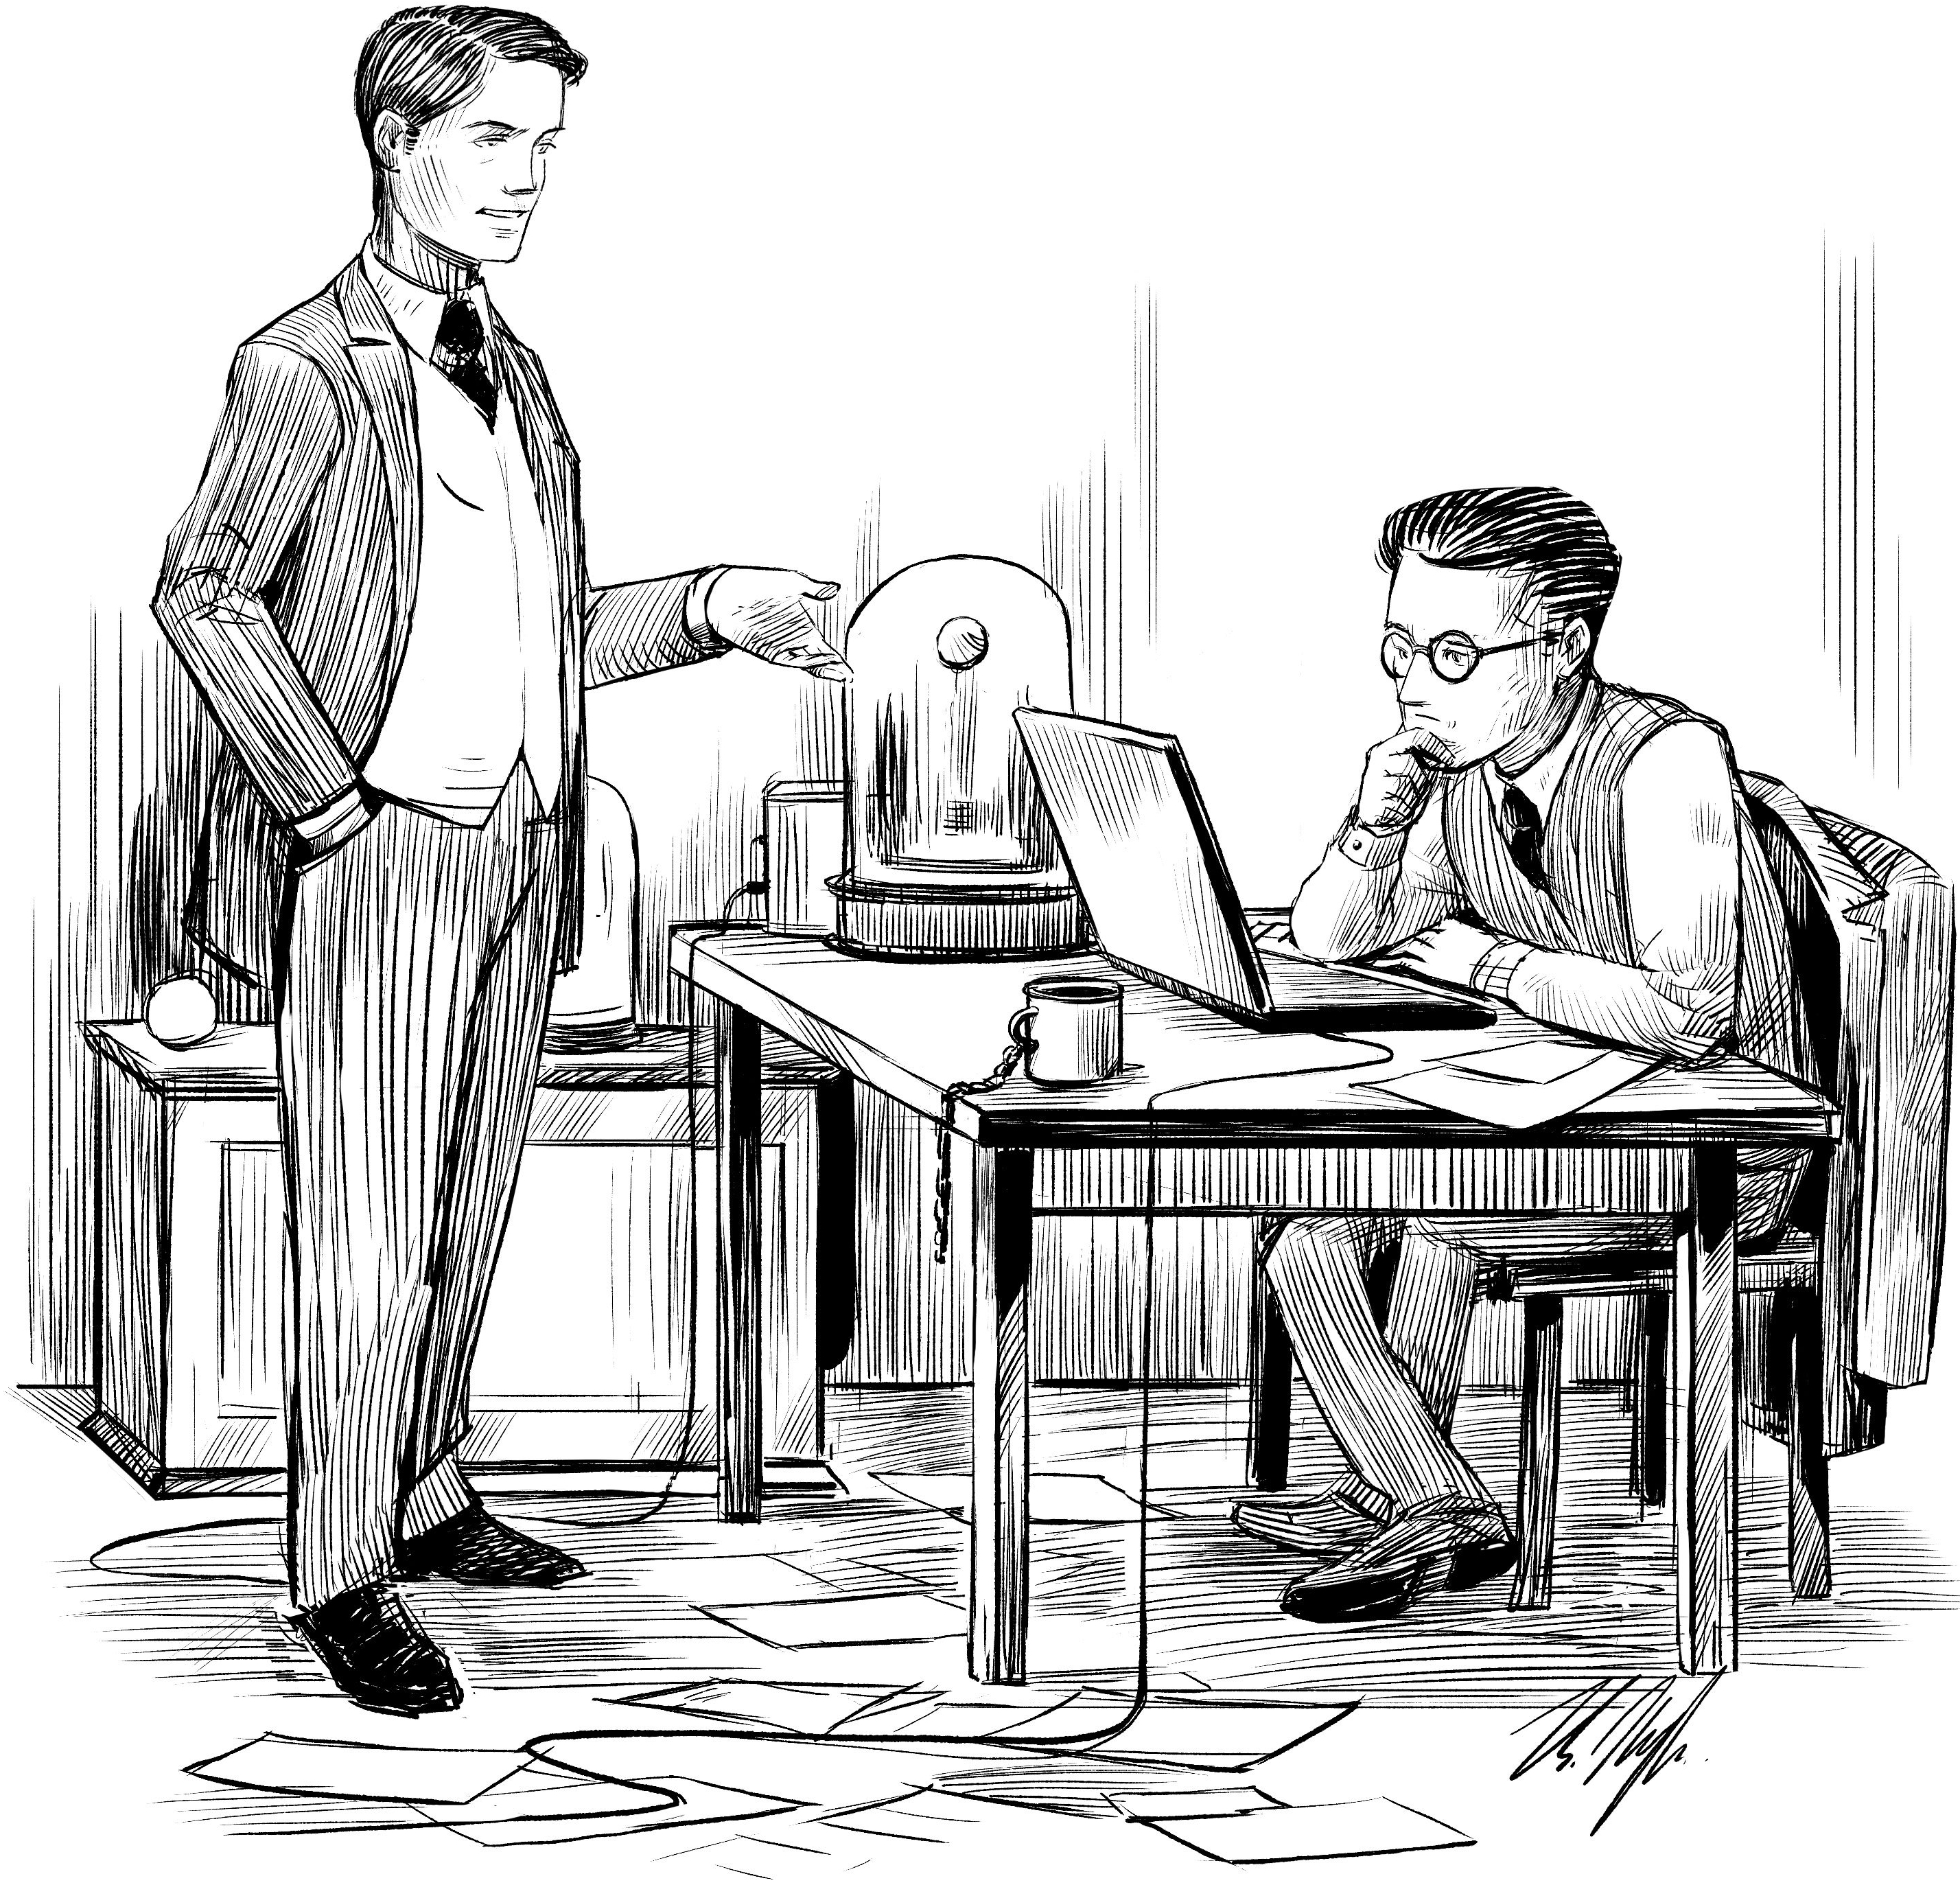
\includegraphics[scale=0.115]{cover.jpg}
\end{center}

Ever since 1931 the main protagonist in any telling of mathematical logic has always been Kurt Gödel and his First Incompleteness Theorem. Roughly speaking this theorem states that any sensible, sufficiently powerful formal system is incomplete; it'll contain a statement that is neither provable nor disprovable.

However, while the statement of the theorem is quite simple, the proof is a very different matter. Entire books, both technical and non-technical, have been devoted to it over the years; some of which, I hope, you'll already be familiar with. Where does this complexity come from? And what can be done about it? These are questions I already addressed in \cite{oberhoff}, though in a rather inexact manner. Indeed, back then I explicitly left important details to ``smarter people'' in the conclusion. Now, some time later, and hopefully a little smarter, I want to return to the question and provide a more precise answer myself.

\section{On ``On Formally Undecidable Propositions''}

To that end let's start with a high-level overview of the famous 1931 paper titled ``On Formally Undecidable Propositions Of Principia Mathematica And Related Systems'' \cite{goedel}. In this paper Gödel dealt with a formal system he had adapted from work by Bertrand Russel and Alfred North Whitehead published in three volumes of the \emph{Principia Mathematica} between 1910 and 1913. This system was based on type theory, a rather tedious framework which has since fallen out of favor. But its salient feature---Peano Arithmetic---has survived in other systems. It defines the natural numbers and is built as follows.

\begin{definition}[Peano Arithmetic]
  The theory of \emph{Peano Arithmetic}, or $\PA$ for short, is defined from the following axioms.
  \begin{description}
    \item[Basic Peano Axioms]
          \begin{description}
            \item[]
            \item[Zero is the first natural number:]
                  $\qu{\forall x \colon \neg\, S x \eq 0}$.
            \item[Successorship is injective:]
                  $\qu{\forall x, y \colon Sx \eq Sy \rightarrow x \eq y}$.
            \item[Induction:]
                  $\qu{(P(0) \land \forall x \colon P(x) \rightarrow P(Sx)) \rightarrow \forall x \colon P(x)}$ for any formula $\qu{P}$.
          \end{description}
    \item[Axioms Of Arithmetic]
          \begin{description}
            \item[]
            \item[Addition:]
                  \begin{align*}
                    \qu{\forall x \colon x + 0}     & \eq\qu{x}        \\
                    \qu{\forall x, y \colon x + Sy} & \eq\qu{S(x + y)}
                  \end{align*}
            \item[Multiplication:]
                  \begin{align*}
                    \qu{\forall x \colon x \times 0}     & \eq\qu{0}                \\
                    \qu{\forall x, y \colon x \times Sy} & \eq\qu{x + (x \times y)}
                  \end{align*}
          \end{description}
  \end{description}
\end{definition}

With all that in mind, here are the major steps in Gödel's 1931 proof:
\begin{description}
  \item[Gödel Numbering:] Akin to modern-day ASCII encoding, Gödel first turned every string and list of strings into a number.
  \item[Computability:] Using the model of computation known as primitive recursive functions Gödel then implemented a proof checker in full detail, showing that $\PA$ is computably enumerable.\footnote{I am in full agreement with Robert I. Soare that ``computably enumerable'' should replace ``recursively enumerable''.}
  \item[Representation:] Next, Gödel briefly pointed out that $\PA$ could represent---that is reason about---primitive recursive functions, and thereby its own proof checker.
  \item[Diagonalization:] Finally, having equipped $\PA$ with the ability of introspection, Gödel diagonalized against provability-in-$\PA$. This produced a sentence asserting its own unprovability, establishing the First Incompleteness Theorem.
\end{description}

This, in essence, is still the argument given to this day. And we're not going to modify its basic structure either. Rather we'll take these items one by one and see where simplifications can be made.

\section{Gödel Numbering}

While today there is an unending variety of computational models, stretching from Diophantine equations to the specification of the Java Virtual Machine, back in 1931 there were only very few available options. That's why when Gödel drew the primitive recursive functions from the shelf the very first challenge he faced was a simple type error. His formal system $\PA$ was built out of strings over an exotic character set whereas primitive recursive functions only mapped natural numbers to natural numbers. If one wanted to devise a proof checker in this model of computation, some type conversion would be unavoidable. So that's exactly what Gödel did using a scheme that since has become known as Gödel numbering. The basic idea will be familiar to anybody who understands the concept of ASCII.

But here's the thing---and this is a point that I really wish was made more often---it's possible to carry out the entire analysis without ever bringing up numbers at all. This is possible since, as already alluded to, Gödel could've picked any model of computation whatsoever for his proof. In particular he could've picked one which mapped strings to strings. Moreover, there's nothing standing in the way of representing such functions in Peano Arithmetic. All that's required is to reinterpret ``$\qu{0}$'' as the empty string and ``$\qu{S}$'' as the lexicographical successor function. The particular choice of alphabetical ordering then becomes the only remaining vestige of Gödel's numbering scheme.

Or, to put it another way, strings already \emph{are} natural numbers.
\begin{definition}[$\mathbb{S}$]
  The set of all strings is denoted $\mathbb{S}$.
\end{definition}
\[
  \mathbb{S} = \{\epsilon, \text{``a''}, \text{``b''}, \dots\} = \mathbb{N}. \tag{$\epsilon$ is the empty string}
\]
All the axioms are met, so it's hard to argue otherwise. Granted, adding or multiplying strings may \emph{feel} disorienting, but surely that's only the fault of our biased upbringing.

However, as enticing as it may be to take this fully unified approach, we won't follow it to the letter here. Having the arity of our functions be strings is just a little too much. What we will do though is that we'll take our computable functions to be mappings from strings to strings. And we'll use the corner quotes usually employed to denote Gödel numbers to point directly to numerals instead.

\begin{definition}
  When handling collections we'll employ boldface variables to avoid clutter. E.g., $\bm{x} \coloneqq x_1, \dots, x_k$.
\end{definition}

\begin{definition}[Numeral]
  Let $x \in \mathbb{S}$. Then
  \[
    \num{x} \enskip\coloneqq\enskip \qu{S \dots S0}
  \]
  where the number of repetitions of $\qu{S}$ indicate the index of $x$ in some enumeration of $\mathbb{S}$. We'll call $\num{x}$ the \emph{numeral} of $x$. Also, when $\bm{x}$ denotes several strings, then $\num{\bm{x}}$ is to be taken element-wise.
\end{definition}

Of course, those who prefer the old way of looking at things are free to ignore this recasting and stick to the conventional ``numeral of Gödel number of''. The proofs will read almost exactly the same.

\section{Computability}

This section is the most notorious in Gödel's original proof. It's a chain of 46 definitions, up to 3 lines each, spread over four pages, altogether implementing a proof checker for $\PA$ using primitive recursive functions.\footnote{Gödel actually gave a relation here, not a function. But that muddles the boundary between the different sections, so I prefer to stick to functions here.} Really though, it's nothing more than an painstaking demonstration that proofs for $\PA$ could be checked by a computer. Let's state this insight more precisely.

\begin{definition}
  $\cmark$ and $\xmark$ can be taken to be arbitrary strings. Their only important feature is that they're distinct.
\end{definition}

\begin{definition}[Proof Checker]
  A function $\pc \colon \mathbb{S}^2 \to \{\cmark, \xmark\}$ is called a \emph{proof checker} for some theory $\T$ if whenever $\T \vdash \qu{A}$, then $\pc(p, \qu{A}) = \cmark$ for some $p \in \mathbb{S}$, and otherwise $\pc(p, \qu{A}) = \xmark$.
\end{definition}

\begin{definition}[Computably Enumerable Theory]
  A theory $\T$ is considered to be \textit{computably enumerable} if there exists a computable proof checker for $\T$.
\end{definition}

\begin{theorem}
  $\Q$ and $\PA$ are computably enumerable theories.
\end{theorem}

\begin{prf}
  Omitted.
\end{prf}

Back in 1931 mathematicians had every right to be doubtful of this claim. This was before we learned of computational universality and familiarized ourselves with higher level languages. Nowadays however this part has become just a routine programming task whose details we won't belabor.

\section{Representation}

Next, we turn to an extremely important section of the proof; the representation of computable functions as formulas. Roughly speaking, for a function $f$ to be represented in a theory $\T$ means that if $f(x) = y$, then $\T$ can prove this fact. And it does so by use of a single formula called ``the representation of $f$''.

\begin{definition}[Representable Function]
  Let $\T$ be a theory containing the first two basic Peano axioms.\footnotemark\ Then a $k$-ary partial function $f \colon \mathbb{S}^k \to \mathbb{S}$ is said to be \emph{represented} in $\T$ if there exists a formula $\rep{f}$ with $k+1$ free variables such that whenever $f(\bm{x}) = y$ then
  \[
    \T \vdash \qu{\exists ! y \colon \rep{f}(\num{\bm{x}}, y)} \quad\text{and}\quad \T \vdash \mathsf{\rep{f}(\num{\bm{x}}, \num{y})}.
  \]
  (Informally: ``$f(\bm{x})$ \emph{only} outputs $y$.'')
\end{definition}
\footnotetext{Without the first two Peano axioms we might not have any such thing as numerals in the first place.}

There are of course many kinds of functions out there which one might want to represent. But for us there's one kind in particular which is of primary concern: the computable functions. A theory which represents all computable functions has in a quite literal sense achieved Turing completeness. It has a fully-fledged programming language embedded within it. And a computable function's representation is none other than its source code. This is why I chose the notation $\rep{f}$, as it's reminiscent of how the code for a Turing machine $M$ is often denoted $\langle M \rangle$. Furthermore, in order to ``execute'' a representation $\rep{f}$ on input $\bm{x}$ one can, for example, go through all possible strings and check if any of them proves a theorem of the form $\rep{f}(\num{\bm{x}}, \num{y})$ for some $y$. If so, $y$ is the output. Naturally, one would hope that this isn't the most efficient way of running a representation. But it proves the point.

This allows us to make the central observation of this section.

\begin{theorem}
  $\Q$ represents every computable function.
\end{theorem}

\begin{prf}
  Omitted.
\end{prf}

The aforementioned result appears in many textbooks on the subject. A particularly accessible demonstration can be found in the publicly available book \textit{Incompleteness and Computability} \cite{zach}. The way I like to think of the situation is that the basic Peano axioms specify what data is. And the axioms of arithmetic delineate a universal gate set from which one can generate any computable function.  What the proof boils down to, therefore, is essentially a tedious exercise in compiler construction. As a matter of fact, even Gödel himself only sketched this part of the argument in his 1931 paper, expounding the details in lectures given in 1934.\footnote{These lectures were attended by Alonzo Church's graduate students Stephen C. Kleene and John B. Rosser. Together they took notes which were first distributed via mimeograph until they were published in 1965 in an anthology by Martin Davis \cite{davis}.}

In broad strokes, one first takes the high-level language used in the rest of the argument---or at least some model of computation one trusts to be universal---and translates it down to a model of computation chosen to be as convenient as possible for Peano Arithmetic to represent. Then one systematically converts every function definable in the chosen model into a formula obeying the definition of representability.

Admittedly, this does open us up to the charge that we're not simplifying much at all over the course of this presentation. We're just moving all the nasty parts out of sight. But I disagree. I think there's real clarity to be won by using the representability of computable functions to impose a clean interface. And in the upcoming section I hope to show that.

\subsection{Representable Terms}

\begin{definition}[Representable Term]
  Let $f$ be represented in $\T$. Then we'll allow ``$f$'' to appear in our formal strings anywhere a regular function symbol could appear. We'll refer to such function symbols as \emph{representable function symbols}. And terms containing representable function symbols are called \emph{representable terms}.

  In order to disabbreviate representable function symbols from some expression we proceed as follows. Let our expression be of the form $\qu{P(\uq{f}(\bm{\qu{r}}))}$ where $\bm{\qu{r}}$ is a collection of regular terms, meaning $f$ is one of the innermost occurrences of a representable function symbol. Then we perform the following expansion:
  \[
    \qu{P(\uq{f}(\bm{\qu{r}}))} \quad\coloneqq\quad \qu{(\exists! y \colon \uq{f}(\bm{\qu{r}}, y)) \leftrightarrow (\exists! y \colon \uq{f}(\bm{\qu{r}}, y) \land P(y))}.
  \]
  And then we continue expanding $\mathsf{P(y)}$ in this way until all representable function symbols have been eliminated.

  Also, it is important that representable terms are expanded \emph{before} newly introduced predicate symbols are.
\end{definition}

That last stipulation is sadly necessary in order to resolve the following ambiguity. Suppose we've defined $\qu{\textscsf{Err}(y)} \coloneqq \qu{\neg\, y = \num{\cmark}}$ and $f$ is some representable function. Then naively $\qu{\textscsf{Err}(\uq{f}(\num{\bm{x}}))}$ might have two possible expansions:
\[
  \underset{\text{(correct)}}{\qu{(\exists! y \colon \rep{f}(\num{\bm{x}}, y)) \leftrightarrow (\exists! y \colon \rep{f}(\num{\bm{x}}, y) \land \neg y = \num{\bm{\cmark}})}} \quad\text{or}\quad \underset{\text{(incorrect)}}{\qu{\neg ((\exists! y \colon \rep{f}(\num{\bm{x}}, y)) \leftrightarrow (\exists! y \colon \rep{f}(\num{\bm{x}}, y) \land  y = \num{\bm{\cmark}}))}}.
\]
To see that these aren't equivalent just imagine $\qu{\exists! y \colon \rep{f}(\num{\bm{x}}, y)}$ was false. Then the left side is true, but the right side is false. Some choice had to be made. And the former struck me as more intuitive and useful. This tripwire is also the reason I'm avoiding the use of $\neq$ in formulas.

\begin{lemma}\label{lm-expd}
  Representable terms expand equivalently in any order.
\end{lemma}

\begin{prf}
  Let's consider the case where we're dealing with just two competing representable function symbols: $\qu{P(\uq{f}(\bm{\qu{r}}), \uq{g}(\bm{\qu{s}}))}$ with $\qu{P}$ being some formula and $\bm{\qu{r}}$ and $\bm{\qu{s}}$ being collections of regular terms. Then the expansions we need to compare are
  \[
    \qu{(\exists! y \colon \uq{f}(\bm{\qu{r}}, y)) \leftrightarrow (\exists! y \colon \uq{f}(\bm{\qu{r}}, y) \land ((\exists! z \colon \uq{g}(\bm{\qu{s}}, z)) \leftrightarrow (\exists! z \colon \uq{g}(\bm{\qu{s}}, z) \land P(y, z))))}\phantom{.}
  \]
  and
  \[
    \qu{(\exists! z \colon \uq{g}(\bm{\qu{r}}, z)) \leftrightarrow (\exists! z \colon \uq{g}(\bm{\qu{r}}, z) \land ((\exists! y \colon \uq{f}(\bm{\qu{s}}, y)) \leftrightarrow (\exists! y \colon \uq{f}(\bm{\qu{s}}, y) \land P(y, z))))}.
  \]
  These can be checked to be equivalent by going through all four combinations of setting $\qu{\exists! y \colon \uq{f}(\bm{\qu{r}}, y)}$ and $\qu{\exists! z \colon \uq{g}(\bm{\qu{s}}, z)}$ to true or false.

  The general case for an arbitrary number of representable terms can then be obtained by observing that any permutation can be decomposed into a series of transpositions.
\end{prf}

\begin{lemma}[Leibniz's Law For Representable Terms]\label{lm-equiv}
  Let $\qu{r}$ and $\qu{s}$ be closed representable terms. And let $\qu{P}$ be a formula with one free variable. Then the following is logically valid:
  \[
    \qu{r \eq s \rightarrow (P(r) \leftrightarrow P(s))}.
  \]
\end{lemma}

\begin{prf}
  By induction on the number of representable function symbols appearing in $\qu{r} \eq \qu{s}$.
  \begin{description}
    \item[Base Case:]
          If $\qu{r}$ and $\qu{s}$ are regular terms, then the statement is trivial.
    \item[Induction:]
          So let's assume that the statement holds for up to $n$ representable functions and that $\qu{r \eq s}$ contains $n + 1$ representable function symbols. Furthermore, without loss of generality let's focus only on the case where $\qu{r}$ contains a representable function symbol, meaning $\qu{r}$ is of the form $\qu{r\qutick}(f(\bm{\qu{t}}))$ for some open representable term $\qu{r\qutick}$ and some collection of closed regular terms $\bm{\qu{t}}$. Then $\qu{r \eq s}$ gives us
          \[
            \qu{(\exists! y \colon \rep{f}(\bm{\qu{t}}, y)) \leftrightarrow (\exists! y \colon \rep{f}(\bm{\qu{t}}, y) \land r\qutick(y) \eq s)}.
          \]
          And what we need to establish is
          \[
            \qu{(\exists! y \colon \rep{f}(\bm{\qu{t}}, y)) \leftrightarrow (\exists! y \colon \rep{f}(\bm{\qu{t}}, y) \land (P(r\qutick(y)) \leftrightarrow P(s)))}.
          \]

          If $\qu{\exists! y \colon \rep{f}(\bm{\qu{t}}, y)}$ is false, then the statement clearly holds. Thus, only the case where $\qu{\exists! y \colon \rep{f}(\bm{\qu{t}}, y)}$ is true remains and our task can be simplified down to show
          \[
            \qu{r\qutick(a) \eq s \rightarrow P(r\qutick(a)) \leftrightarrow P(s)}
          \]
          where $\qu{a}$ is the unique object such that $\qu{\rep{f}(\bm{\qu{t}}, a)}$. At this stage, $\qu{r\qutick(a) = s}$ is closed and contains only $n$ representable function symbols. So we can bring the inductive hypothesis to bear, immediately concluding the argument.\qedhere
  \end{description}
\end{prf}

\begin{lemma}[Rules Of Equality For Representable Terms]\label{lm-eq}
  Let $\qu{r, s}$, and $\qu{t}$ be closed representable terms. Then the rules of equality for representable terms are logically valid.
  \begin{description}[leftmargin=!, labelwidth=\widthof{Transitivity:}]
    \item[Reflexivity:] $\qu{r \eq r}$.
    \item[Symmetry:] $\qu{r \eq s \rightarrow s \eq r}$.
    \item[Transitivity:] $\qu{r \eq s \rightarrow (s \eq t \rightarrow r \eq t)}$.
  \end{description}
\end{lemma}

\begin{prf}
  \phantom{}
  \begin{description}
    \item[Reflexivity:]
          By induction on the number of representable function symbols appearing in $\qu{r \eq r}$.
          \begin{description}
            \item[Base Case:]
                  If $\qu{r}$ is a regular term, then the regular reflexivity rule applies.
            \item[Induction:]
                  Expanding out one of the innermost representable function symbols turns $\qu{r \eq r}$ into
                  \[
                    \qu{(\exists! y \colon \rep{f}(\bm{\qu{t}}, y)) \leftrightarrow (\exists! y \colon \rep{f}(\bm{\qu{t}}, y) \land ((\exists! z \colon \rep{f}(\bm{\qu{t}}, z)) \leftrightarrow (\exists! z \colon \rep{f}(\bm{\qu{t}}, z) \land r\qutick(y) = r\qutick(z))))}
                  \]
                  where $\qu{r\qutick}$ is an open representable term and $\bm{\qu{t}}$ is a collection of closed regular terms. This is evidently true if $\qu{\exists! y \colon \rep{f}(\bm{\qu{t}}, y)}$ false. And if $\qu{\exists! y \colon \rep{f}(\bm{\qu{t}}, y)}$ is true, then the statement reduces to $\qu{r\qutick(a) \eq r\qutick(a)}$ where $\qu{a}$ is the unique object such that $\qu{\rep{f}(\bm{\qu{t}}, a)}$. And this is true by inductive hypothesis.
          \end{description}
    \item[Symmetry:]
          By Leibniz's Law we have $\qu{r \eq s \rightarrow (s \eq r \leftrightarrow r \eq r)}$ which reduces to $\qu{r \eq s \rightarrow s \eq r}$ by reflexivity.
    \item[Transitivity:]
          Once again, by Leibniz's Law we have $\qu{r \eq s \rightarrow (s \eq t \leftrightarrow r \eq t)}$ which implies the desired statement.\qedhere
  \end{description}
\end{prf}

\begin{lemma}[Runtime Lemma]\label{lm-is}
  Let $f$ be a function which is represented in $\T$. And suppose $f(\bm{x}) = y \neq z$. Then
  \[
    \T \vdash f(\num{\bm{x}}) \eq \num{y} \quad\text{and}\quad \T \vdash \neg f(\num{\bm{x}}) \eq \num{z}.
  \]
\end{lemma}

\begin{prf}
  After expanding notation and minor simplification $f(\num{\bm{x}}) = \num{y}$ can be turned into
  \[
    \qu{(\exists ! y \colon \rep{f}(\num{\bm{x}}, \mathsf{y})) \leftrightarrow \rep{f}(\num{\bm{x}}, \num{y})},
  \]
  both halves of which $\T$ can prove by the definition of representable functions. This also allows $\T$ to disprove $f(\num{\bm{x}}) = \num{z}$ since if it were true, then by transitivity we'd have $\num{y} = \num{z}$. And that is false by the first two Peano axioms alone.
\end{prf}


\section{Diagonalization}

\begin{definition}
  Writing $A(\rep{f})$ in the signature of an algorithm $A$ means that $A$ expects a representation as input, akin to pattern matching. For invalid inputs (which we'll avoid) the algorithm is allowed to arbitrarily misbehave.
\end{definition}

\begin{lemma}[Diagonal Lemma]
  Let $\T$ be a theory which represents every computable function. And let $\qu{P}$ be a formula with one free variable. Then there exists a sentence $\qu{A}$ referred to as a ``fixed point'' such that $\T \vdash \qu{A} \leftrightarrow \qu{P}(\num{\qu{A}})$.
\end{lemma}

\begin{prf}
  Consider the following algorithm.
  \begin{algo}
    \Function{$D(\rep{f})$}{}
    \State\Return $\qu{P}(f(\numrep{f}))$
    \EndFunction
  \end{algo}
  Then $\T \vdash D(\numrep{D}) = \num{\mathsf{P}(D(\numrep{D}))}$ by the Runtime Lemma and hence $\T \vdash \mathsf{P}(D(\numrep{D})) \leftrightarrow \mathsf{P}(\num{\mathsf{P}(D(\numrep{D}))})$ by Leibniz's Law, giving fixed point $\mathsf{P}(D(\numrep{D}))$.
\end{prf}

The main use of the Diagonal Lemma is to produce the Gödel sentence. Consider the following predicate.
\begin{definition}[$\Pvb_\mathsf{G}$]
  Let $\T$ be a computably enumerable theory which represents every computable function. Then
  \[
    \qu{\Pvb_G(x) \enskip\coloneqq\enskip \exists p \colon \pc(p,x) = \num{\cmark}}
  \]
  where $\pc$ is a proof checker for $\T$.
\end{definition}
Then if one applies the Diagonal Lemma to $\neg \Pvb_{\mathsf{G}}$, one produces a sentence $\mathsf{G}$ such that $\T$ proves $\mathsf{G} \leftrightarrow \neg\Pvb_{\mathsf{G}}(\num{\mathsf{G}})$. Informally this sentence states: ``I am not provable.'' which, assuming that $\T$ is consistent, turns out to be true. Furthermore, one can also show that $\neg \mathsf{G}$ can't be provable either. Though this needs the stronger assumption that $\T$ is \emph{correct}; if $\T$ proves something, then it is actually so. Or at least it requires $\omega$-consistency; if $\T$ proves that some unbounded search terminates, then it actually does. So in summary, if $\T$ is $\omega$-consistent, computably enumerable, and represents every computable function, it is incomplete.

For the audience in 1931 this already settled the matter. Still, in 1936 John B. Rosser found a way to iron out the last wrinkle as well by using this predicate instead \cite{rosser}:
\begin{definition}[String Concatenation]
  $\ast$ is the computable function which concatenates two strings. Furthermore, we'll use left-associative infix notation for this function, so $x \ast y \ast z \coloneqq ((x \ast y) \ast z)$. The fact that this function is associative won't be needed.
\end{definition}

\begin{definition}[$\Pvb_{\mathsf{R}}$]
  Let $\T$ be a computably enumerable extension of $\Q$. Then
  \[
    \qu{\Pvb_R(x) \enskip\coloneqq\enskip \exists p \colon \pc(p, x) = \num{\cmark} \land \forall q < p \colon \neg \pc(q, \num{\neg} \ast x) = \num{\cmark}}
  \]
  where $\pc$ is a proof checker for $\T$.
\end{definition}
If one applies the Diagonal Lemma to $\neg\Pvb_{\mathsf{R}}$, it produces the Rosser sentence $\mathsf{R}$ which can be paraphrased as: ``For every proof of me there exists a shorter disproof.'' This sentence, unlike $\mathsf{G}$, can be demonstrated to be neither provable nor disprovable assuming only the consistency of $\T$, giving us the much nicer formulation: if $\T$ is a consistent and computably enumerable extension of $\Q$, it is incomplete.

Rosser's argument only comes with the minor drawback that just to have $<$ available one already has to narrow the discussion from theories which represent every computable function to just extensions of $\Q$. And one also still has spell out a few more details. For starters, one has to first establish the following lemma.
\begin{lemma}\label{lm-count}
  For any formula $\qu{P}$ and numeral $\mathsf{n}$:
  \[
    \Q \vdash \qu{(\forall x < Sn \colon P(x)) \leftrightarrow (P(0) \land P(1) \land \dots \land P(n))}.
  \]
\end{lemma}

\begin{prf}
  Omitted.
\end{prf}

This brings us then to another way of proving the First Incompleteness Theorem which in my mind fully captures the essence with wonderful concision.
\begin{theorem}[First Incompleteness Theorem]\label{tm-first}
  Let $\T$ be a consistent and computably enumerable theory which represents every computable function. Then $\T$ is incomplete.
\end{theorem}

\begin{prf}
  First, we construct the following algorithm.
  \begin{algo}
    \Function{$X(\rep{f})$}{}
    \For{$p \in \mathbb{S}$}
    \If{$p$ proves $\neg f(\numrep{f}) \eq \num{\cmark}$}
    \State\Return \hspace{-1.8pt} $\cmark$
    \EndIf
    \vspace{-2.75pt}
    \If{$p$ proves $\hphantom{\neg}f(\numrep{f}) \eq \num{\cmark}$}
    \State\Return \hspace{-1.8pt} $\xmark$
    \EndIf
    \EndFor
    \EndFunction
  \end{algo}
  This lets us produce
  \[
    \mathsf{R} \enskip\coloneqq\enskip \neg X(\numrep{X}) \eq \num{\cmark}.
  \]
  Now suppose that $\mathsf{R}$ was decidable. Then there must exist a \emph{first} $p \in \mathbb{S}$ which decides $\mathsf{R}$. This leads to two cases.
  \newline
  \begin{minipage}{0.46\textwidth}
    \smallskip
    \begin{description}[leftmargin=0.5cm]
      \item[$p$ proves $\mathsf{R}$:]
            Then $X(\rep{X})$ returns $\cmark$ upon finding $p$ and so $\T \vdash \neg \mathsf{R}$ by Lemma \ref{lm-is}, an inconsistency.
    \end{description}
  \end{minipage}
  \hspace{0.06\textwidth}
  \begin{minipage}{0.46\textwidth}
    \smallskip
    \begin{description}[leftmargin=0.5cm]
      \item[$p$ proves $\neg \mathsf{R}$:]
            Then $X(\rep{X})$ returns $\xmark$ upon finding $p$ and so $\T \vdash \mathsf{R}$ by Lemma \ref{lm-is}, an inconsistency.\qedhere
    \end{description}
  \end{minipage}
\end{prf}

The sentence $\mathsf{R}$ used in the above proof carries its name for a reason. It's because, as some reflection will reveal, $\mathsf{R}$ is indeed a Rosser sentence, claiming: ``For every proof of me there exists a shorter disproof.'' Furthermore, in order to recover the original ``I am not provable'' one only needs to drop the last two lines of $X$. This is also the reason I set up $\mathsf{R}$ and $\neg \mathsf{R}$ the way I did and not the other way around, despite this introducing the minor subtlety that $\neg \mathsf{R}$ denotes $\mathsf{R}$ with a negation sign removed rather than added.

\section{Re-Representation}

At a high level the Second Incompleteness Theorem isn't all that hard to grasp. We've already seen that if our theory is consistent, then $\mathsf{G}$ isn't provable and thereby true. In short, $\Con \rightarrow \mathsf{G}$ where $\Con$ expresses the consistency of the theory. What's more, as Gödel first noted in 1931, this fact can be proved in a theory such as $\PA$ as well since it can step through the proof of the First Incompleteness Theorem just the same. To coin a phrase, $\PA$ represents that it represents---or \emph{re-represents}---its own proof checker. But that means that if $\PA$ could prove $\Con$, then $\PA$ could also prove $\mathsf{G}$ by modus ponens which is impossible. Whence the Second Incompleteness Theorem: if $\PA$ is consistent, then it can't prove this to be so.

Alas, the crucial fact that $\Con \rightarrow \mathsf{G}$ can be proved in $\PA$ is notoriously difficult to establish rigorously. Gödel himself famously concluded his 1931 paper stating: ``The results will be stated and proved in fuller generality in a forthcoming sequel. There too, the mere outline proof we have given of [the Second Incompleteness Theorem] will be presented in detail.'' Such a sequel never came. Instead, the first rigorous demonstration appeared in 1939 in the second volume of \textit{Foundations of Mathematics} written by David Hilbert and his assistant Paul Bernays---Bernays being the main author.

But besides technical issues, there are also conceptual ones. Most importantly, what exact expression should we choose for $\Con$? Gödel had the obvious in mind:
\begin{definition}[$\Con_{\mathsf{G}}$]
  \hspace{2.25cm}$\Con_{\mathsf{G}} \enskip\coloneqq\enskip \mathsf{\neg \exists a \colon \Pvb_{\mathsf{G}}(a) \land \Pvb_{\mathsf{G}}(\num{\neg} \ast a)}$
\end{definition}
However, Gödel had many freedoms when making his construction. What made the choice he arrived at the right one? This question is brought to a head when one examines the alternative derived from Rosser's predicate.
\begin{definition}[$\Con_{\mathsf{R}}$]
  \hspace{2.25cm}$\Con_{\mathsf{R}} \enskip\coloneqq\enskip \mathsf{\neg \exists a \colon \Pvb_{\mathsf{R}}(a) \land \Pvb_{\mathsf{R}}(\num{\neg} \ast a)}$
\end{definition}
If one were to use this consistency statement instead, then the theory actually \emph{could} prove its own consistency. This happens for the simple reason that \emph{every} theory, whether consistent or not, is ``consistent'' according to the Rosser definition.

To answer all this history eventually decided to put down three conditions that any provability predicate ought to meet.

\begin{definition}[Derivability Conditions]
  A predicate $\Pvb$ obeys the \emph{derivability conditions} for a theory $\T$ if the following holds for any sentences $\mathsf{A}, \mathsf{B}$:
  \begin{description}[leftmargin=!, labelwidth=\widthof{Re-Representability:}]
    \item[Representability:]
          If $\T \vdash \mathsf{A}$, then $\T \vdash \Pvb(\num{\mathsf{A}})$.
    \item[Distributivity:]
          $\T \vdash \Pvb(\num{\mathsf{A \rightarrow B}}) \rightarrow (\Pvb(\num{\mathsf{A}}) \rightarrow \Pvb(\num{\mathsf{B}}))$.
    \item[Re-Representability:]
          $\T \vdash \Pvb(\num{\mathsf{A}}) \rightarrow \Pvb(\num{\Pvb(\num{\mathsf{A}})})$.
  \end{description}
\end{definition}

From these three conditions---also known as the HBL-derivability conditions (Hilbert, Bernays, Löb)---the Second Incompleteness Theorem can be derived in short order. This both shuts the door on Rosser's predicate and provides a convenient layer of abstraction, similar to the representability of computable functions.

The only question left on the table is then: does some proposed provability predicate actually meet the criteria? This is where all the fearsome details end up hiding. The standard approach using $\PA$'s $\Pvb_\qu{G}$ runs roughly as follows.
\begin{description}
  \item[Representability:]
        This part carries over from the proof of the First Incompleteness Theorem and is basically free.
  \item[Distributivity:]
        Here one can show that $\PA$ recognizes the modus ponens inference rule in $\Pvb_\qu{G}$. That is to say, $\PA$ can prove a concatenation of a proof of $\mathsf{A}$, a proof of $\mathsf{A \rightarrow B}$, and the list containing only $\mathsf{B}$ to be a proof of $\mathsf{B}$. Doing so requires some cursory inspection of $\Pvb_\qu{G}$ as well as wading through a fair number of details involving elementary features of lists. But it's still manageable.
  \item[Re-Representability:]
        This is the true villain of the story. In outline the strategy is to show that
        \[
          \PA \vdash \qu{(\exists x \colon P(x)) \rightarrow \Pvb_G(\num{\qu{\exists x \colon P(x)}})}
        \]
        for any formula $\mathsf{P}$ of one free variable built without unbounded quantifiers. Since $\Pvb_{\mathsf{G}}(\num{\mathsf{A}})$ can be written in this form that proves the claim. But checking the above demands an exceedingly elaborate structural induction on the construction of $\mathsf{P}$, during each stage of which one has to examine the inner details of $\Pvb_\qu{G}$. And if that wasn't enough, realize that as soon as one moves on from $\PA$ to any of its extensions one is presented with a new provability predicate for that theory and one has to start all over again.
\end{description}

The challenge ahead of us is daunting. So instead of charging straight ahead let's pause for a moment and try to figure out what is fundamentally causing the difficulty. It's that, whereas the modus ponens inference rule is typically coded into $\Pvb_{\mathsf{G}}$ at a high level, the re-representability property emerges piece by piece from the entirety of the construction. But picking $\Pvb_{\mathsf{G}}$ as our provability predicate was a deliberate choice; a choice which we can amend. If only we could find a provability predicate which carried the re-representability property at the surface, then we might save ourselves a lot of grief during the verification.

Indeed, why not simply pick the following provability predicate and declare victory?
\[
  \mathsf{\Pvb_\top(x) \enskip\coloneqq\enskip x = x}
\]
This predicate trivially satisfies all three conditions. Yet something is clearly amiss here. According to $\Pvb_\top$ everything is provable. In other words, $\Pvb_\top$ encodes the belief that our theory is inconsistent. Yes, the Second Incompleteness Theorem still applies to this predicate. But it has degenerated into the trite observation that a consistent theory which believes itself to be inconsistent can't simultaneously assert its own consistency. Evidently we're still missing something basic.

\begin{definition}[Provability Predicate]
  A predicate $\Pvb$ is considered a \emph{provability predicate} for a theory $\T$ if it obeys the following condition.
  \begin{description}
    \item[Correctness:] $\Pvb(\num{\mathsf{A}})$ is true (in the intended interpretation) if and only if $\T \vdash \mathsf{A}$.
  \end{description}
\end{definition}

\begin{definition}[Weak Provability Predicate]
  A predicate $\Pvb$ is considered a \emph{weak} or \emph{representable provability predicate} for a theory $\T$ if it is a provability predicate which also obeys the following condition.
  \begin{description}
    \item[Representability:] If $\T \vdash \mathsf{A}$, then $\T \vdash \Pvb(\num{\mathsf{A}})$.
  \end{description}
\end{definition}

\begin{definition}[Strong Provability Predicate]
  A predicate $\Pvb$ is considered a \emph{strong provability predicate} for a theory $\T$ if it is a provability predicate which also obeys the derivability conditions.
\end{definition}

Assembling a predicate with the correctness property all the way from scratch would take a while. So let me set up an intermediate abstraction to build on top of.

\begin{definition}[Correctly Representable Function]
  A function $f$ is considered to be \textit{correctly represented} in a theory $\T$ if it is represented in $\T$ by a formula $\rep{f}$ and $\rep{f}(\num{\bm{x}}, \num{y})$ is true if and only if $f(\bm{x}) = y$.
\end{definition}
The following should then come with little surprise.
\begin{theorem}
  $\Q$ correctly represents every computable function.
\end{theorem}

\begin{prf}
  Omitted.
\end{prf}
All that's required for this result is to retrace the argument by which $\Q$ represents every computable function and check that correctness is satisfied at each step.

It's also worth bearing in mind that the ability of a theory $\T$ to correctly represent a function by no means implies that $\T$ is a correct theory. For instance, since $\Q$ correctly represents every computable function so does every extension of it, including the inconsistent ones.

We can then already check off two of the first two boxes.
\begin{lemma}\label{lm-cpvb}
  Let $\T$ be a theory which correctly represents every computable function. Then $\Pvb_\mathsf{G}$ is a weak provability predicate (provided it has been built with a correct representation of $\pc$).
\end{lemma}

\begin{prf}
  Simply set
  \[
    \mathsf{\Pvb(a)  \enskip\coloneqq\enskip \exists p \colon \pc(p,a) = \num{\cmark}}
  \]
  using a correct representation of $\T$'s proof checker $\pc$. Then completeness follows immediately from Lemma \ref{lm-1}. And correctness is satisfied since, in one direction, if $\Pvb(\num{\mathsf{A}})$ is true, then there exists a $p \in \mathbb{S}$ such that $\pc(\num{p}, \num{\mathsf{A}}) = \num{\cmark}$ is true.\footnote{This step relies on our convention that $\num{\cdot}$ denotes numerals directly and is therefore bijective. A merely injective Gödel numbering would require more care.} This implies $\pc(p, \mathsf{A}) = \cmark$ and hence $\T$ proves $\mathsf{A}$. And in the other direction, if $\T$ proves $\mathsf{A}$, then there exists a $p \in \mathbb{S}$ such that $\pc(p, \mathsf{A}) = \cmark$. So $\pc(\num{p}, \num{\mathsf{A}}) = \num{\cmark}$ is true and so is $\Pvb(\num{\mathsf{A}})$.
\end{prf}

So far so good. But now for the heart of the matter: can we find a \emph{strong} provability predicate which is also easily recognized as such? As a matter of fact we can, starting with the following idea.

Take a closer look at this example consequent of the re-representability condition: $\Pvb(\num{\Pvb(\num{\mathsf{S0 + S0 = SS0}})})$. Antropomorphizing our provability predicate lets us rephrase this in English as: ``Do you believe that you believe that $1 + 1 = 2$?'' Now answer me this: if you were ever asked this question yourself, would you then dutifully proceed to simulate your own brain as it is pondering whether $1 + 1 = 2$? I doubt it. More likely you'd just ponder the question directly. But then why not permit $\Pvb$ the same liberty? That is to say, why couldn't $\mathsf{A}$ be used to derive $\Pvb(\num{\mathsf{A}})$ straight away? In customary notation we'll then have these two inference rules built into our proof checker:
\[
  \text{Modus Ponens:}\quad\frac{\mathsf{A} \qquad \mathsf{A \rightarrow B}}{\mathsf{B}} \hspace{3cm} \text{Representability:}\quad\frac{\mathsf{A}}{\Pvb(\num{\mathsf{A}})}
\]
We're going to have to meet the completeness condition---if $\mathsf{A}$ is a theorem, so is $\Pvb(\num{\mathsf{A}})$---anyway. So this is a completely sound inference to make. The only puzzle this leaves us with is to find a way for $\Pvb$ to recognize itself. But at this point that's a well-practiced routine. The solution, as usual, is to run a program on its own source code.

Also, I want to remark that I did toy with more general framings of the upcoming result. But those attempts all turned out overly cumbersome. So instead I've chosen to make a few more hopefully uncontroversial assertions about $\PA$ and go from there.

\begin{definition}[List]
  A \emph{list} is a single string which contains a finite ordered set of other strings via some coding. Furthermore, we'll write $[\bm{x}]$ to denote the list whose items are $\bm{x}$. Strictly speaking, this is an infinite set of computable functions, one for each number of inputs. So there are $[\cdot], [\cdot, \cdot]$, $[\cdot, \cdot, \cdot]$, etc.
\end{definition}

\begin{definition}[List Item Retrieval]
  Further extending our use of computer programming notation we'll use $\cdot[\cdot]$ to denote the computable function which given a list $[\bm{x}]$ and index $i$ retrieves the $i$th item of $[\bm{x}]$, namely $x_i$. In short: $[\bm{x}][i] = x_i$.
\end{definition}

\begin{definition}[List Length]
  $\lVert \cdot \rVert$ denotes the computable function which determines the length of a list.
\end{definition}

\begin{definition}[List Concatenation]
  $\bast$ denotes the computable function which concatenates two lists. And analogously to string concatenation we'll use left-associative infix notation for this function.
\end{definition}

Side note: I considered setting things up so that string and list concatenation coincided, but that too seemed to cause more trouble than it was worth.

\begin{lemma}\label{lm-cat}
  $\PA$ proves the following theorems for some correct representations of $\cdot[\cdot]$, $\lVert \cdot \rVert$, and $\bast$.
  \begin{align*}
     & \mathsf{\forall a, b \colon \forall i < \lVert a \rVert \colon a[i] = (a \bast b)[i]}                   \\
     & \mathsf{\forall a, b \colon \forall i < \lVert b \rVert \colon b[i] = (a \bast b)[\lVert a \rVert + i]} \\
     & \mathsf{\forall a, b \colon \lVert a \bast b \rVert = \lVert a \rVert + \lVert b \rVert}
  \end{align*}
\end{lemma}

\begin{prf}
  Omitted.
\end{prf}

\begin{theorem}[Existence Theorem For Strong Provability Predicates]
  Let $\T$ be a computably enumerable theory containing $\PA$. Then there exists a strong provability predicate for $\T$.
\end{theorem}

\begin{prf}
  By virtue of $\T$ being computably enumerable and containing $\PA$ we can employ Lemma \ref{lm-cpvb} to provide us with a predicate $\Pvbp$ already equipped with the completeness and correctness properties. We can then bolt on the modus ponens and reflection properties by first constructing the following algorithm.
  \begin{algo}
    \Function{$Q(\rep{f}, x)$}{}
    \State\Return $\begin{aligned}[t]
        \mathsf{\exists p, z \colon} & \mathsf{p[z]} = \num{x} \, \land                \\
                                     & \lVert \mathsf{p} \rVert = \mathsf{Sz} \, \land \\
                                     & \mathsf{\forall i < \lVert p \rVert \colon}
        \begin{aligned}[t]
           & \mathsf{\Pvbp(p[i]) \, \lor}     \\
           & \mathsf{\exists j, k < i \colon}
          \begin{aligned}[t]
             & \mathsf{p[k] = p[j] \ast \num{\rightarrow} \ast p[i] \, \lor} \\
             & \mathsf{p[i] = \mathit{f}(\numrep{f}, p[j])}
          \end{aligned}
        \end{aligned}
      \end{aligned}$
    \EndFunction
  \end{algo}
  And then we have the accompanying provability predicate:
  \[
    \Pvb(\mathsf{a}) \enskip\coloneqq\enskip
    \begin{aligned}[t]
      \mathsf{\exists p, z \colon} & \mathsf{p[z] = a} \, \land                      \\
                                   & \lVert \mathsf{p} \rVert = \mathsf{Sz} \, \land \\
                                   & \mathsf{\forall i < \lVert p \rVert \colon}
      \begin{aligned}[t]
         & \mathsf{\Pvbp(p[i]) \, \lor}     \\
         & \mathsf{\exists j, k < i \colon}
        \begin{aligned}[t]
           & \mathsf{p[k] = p[j] \ast \num{\rightarrow} \ast p[i] \, \lor} \\
           & \mathsf{p[i] = \mathit{Q}(\numrep{Q}, p[j])}
        \end{aligned}
      \end{aligned}
    \end{aligned}\tag*{\parbox[t]{7cm}{\raggedleft\footnotesize (there exists a proof $\mathsf{p}$ containing $\mathsf{a}$)                                                                               \\[5pt] ($\mathsf{a}$ is the last line)\\[5pt] (every line of $\mathsf{p}$ is either $\Pvbp$-provable)\\[5pt] (or follows by modus ponens)\\[5pt] (or follows by representability)}}
  \]

  Onwards to the verfication.
  \begin{description}
    \item[Representability:]
          If $\mathsf{A}$ is provable, then $\mathsf{[A]}$ by itself already constitutes a ``proof'' and we're naturally led to the claim
          \[
            \num{[\mathsf{A}]}[\mathsf{0}] = \num{\mathsf{A}} \land \mathsf{\lVert \num{\mathsf{[A]}} \rVert = S0 \land \forall i < \lVert \num{[\mathsf{A}]} \rVert \colon \Pvbp(\num{[\mathsf{A}]}[i])}
          \]
          which can be seen to be provable through applications of Lemmas \ref{lm-1}, \ref{lm-2}, \ref{lm-count}, and the completeness property of $\Pvbp$. The desired conclusion $\Pvb(\num{\mathsf{A}})$ follows without effort.
    \item[Distributivity:]
          Here we need to establish that $\T$ can argue from the assumptions $\Pvb(\num{\mathsf{A}})$ and $\Pvb(\num{\mathsf{A \rightarrow B}})$ to the conclusion $\Pvb(\num{\mathsf{B}})$. More concretely, we'll want to show that if we instantiate the two existentials $\Pvb(\num{\mathsf{A}})$ and $\Pvb(\num{\mathsf{A \rightarrow B}})$ with $\mathsf{p_A}$ and $\mathsf{p_{A \imp B}}$ respectively, then $\mathsf{p_A \bast p_{A \imp B} \bast \num{[\mathsf{B}]}}$ will be able to serve as a witness for $\Pvb(\num{\mathsf{B}})$.

          To this end we begin by using Lemma \ref{lm-cat} to obtain $\mathsf{p_{B{\textbf\textquotesingle}}, p_B}$, and $\mathsf{z_B}$ such that
          \[
            \mathsf{p_{B{\textbf\textquotesingle}} = p_A \bast p_{A \imp B} \qquad\text{and}\qquad p_B = p_{B{\textbf\textquotesingle}} \bast \num{[\mathsf{B}]} \qquad\text{and}\qquad z_B = \lVert p_{B{\textbf\textquotesingle}} \rVert}.
          \]
          We now take the conjuncts of $\Pvb(\num{\mathsf{B}})$ in turn.
          \begin{description}
            \item[$\mathsf{p_B[z_B] = \num{\mathsf{B}}}$:]
                  \[
                    \mathsf{p_B[z_B] = (p_{B{\textbf\textquotesingle}} \bast \num{[\mathsf{B}]})[\lVert p_{B{\textbf\textquotesingle}} \rVert + 0]} = \num{[\mathsf{B}]}[0] = \num{\mathsf{B}}.
                  \]
            \item[$\mathsf{\lVert p_B \rVert = Sz_B}$:]
                  \[
                    \mathsf{\lVert p_B \rVert = \lVert p_{B{\textbf\textquotesingle}} \rVert + \lVert \num{[\mathsf{B}]} \rVert = Sz_B}.
                  \]
            \item[$\mathsf{\forall i < \lVert p_B \rVert \colon \Pvbp(p_B[i]) \;\lor\; \exists j, k < i \colon\; p_B[k] = p_B[j] \ast \num{\rightarrow} \ast p_B[i] \;\lor\; p_B[i] = \mathit{Q}(\numrep{Q}, p_B[j])}$:]
                    What's left then is to verify that $\T$ can prove every line of $\mathsf{p_B}$ to be valid. An assumption which can be turned into $\mathsf{i \leq \lVert p_A \rVert + \lVert p_{A \imp B} \rVert}$ and then broken down into three cases.
                  \begin{description}
                    \item[$\mathsf{i < \lVert p_A \rVert}$:]
                          Using Lemmas \ref{lm-2} and \ref{lm-cat} repeatedly allows $\T$ to carry out the following conversion:
                          \[
                            \begin{aligned}
                               & \mathsf{\Pvbp(p_A[i]) \, \lor}   \\
                               & \mathsf{\exists j, k < i \colon}
                              \begin{aligned}[t]
                                 & \mathsf{p_A[k] = p_A[j] \ast \num{\rightarrow} \ast p_A[i] \, \lor} \\
                                 & \mathsf{p_A[i] = \mathit{Q}(\numrep{Q}, p_A[j])}
                              \end{aligned}
                            \end{aligned}
                            \qquad\leftrightarrow\qquad
                            \begin{aligned}
                               & \mathsf{\Pvbp(\mathsf{p_B}[i]) \, \lor} \\
                               & \mathsf{\exists j, k < i \colon}
                              \begin{aligned}[t]
                                 & \mathsf{\mathsf{p_B}[k] = \mathsf{p_B}[j] \ast \num{\rightarrow} \ast \mathsf{p_B}[i] \, \lor} \\
                                 & \mathsf{\mathsf{p_B}[i] = \mathit{Q}(\numrep{Q}, \mathsf{p_B}[j])}
                              \end{aligned}
                            \end{aligned}\enskip;
                          \]
                          of course having obtained the left-hand side from $\Pvb(\num{\mathsf{A}})$. Let's consider an example to illustrate: the substitution of $\mathsf{p_A[k]}$ on the left with $\mathsf{p_B[k]}$ on the right. Suppose we had instantiated $\mathsf{k}$ on the left with $\mathsf{k_A}$. Then since $\mathsf{k_A < i} < \lVert \mathsf{p_A} \rVert < \lVert \mathsf{p_A \bast p_{A \imp B}} \rVert$ we can use Lemma \ref{lm-cat} to deduce
                          \[
                            \mathsf{p_A[k_A] = (p_A \bast p_{A \imp B})[k_A] = p_{B{\textbf\textquotesingle}}[k_A] = (p_{B{\textbf\textquotesingle}} \bast \num{[\mathsf{B}]})[k_A] = p_B[k_A]}.
                          \]
                          And at that point Lemma \ref{lm-2} yields the desired equivalency. The other cases are virtually identical.
                          % \item[$\mathsf{\lVert p_A \rVert \leq i < \lVert p_A \rVert + \lVert p_{A \imp B} \rVert}$:]
                          Here we evidently have $\mathsf{i} = \lVert \mathsf{p_A} \rVert + \mathsf{i_{A \imp B}}$ for some $\mathsf{i_{A \imp B}} < \lVert \mathsf{p_{A \imp B}} \rVert $ which allows us to employ Lemmas \ref{lm-2} and \ref{lm-cat} in much the same way as last time to convert
                          \[
                            \begin{aligned}
                               & \mathsf{\Pvbp(p_{A \imp B}[i_{A \imp B}]) \, \lor} \\
                               & \mathsf{\exists j, k < i_{A \imp B} \colon}
                              \begin{aligned}[t]
                                 & \mathsf{p_{A \imp B}[k] = p_{A \imp B}[j] \ast \num{\rightarrow} \ast p_{A \imp B}[i_{A \imp B}] \, \lor} \\
                                 & \mathsf{p_{A \imp B}[i_{A \imp B}] = \mathit{Q}(\numrep{Q}, p_{A \imp B}[j])}
                              \end{aligned}
                            \end{aligned}
                            \qquad\leftrightarrow\qquad
                            \begin{aligned}
                               & \mathsf{\Pvbp(\mathsf{p_B}[i]) \, \lor} \\
                               & \mathsf{\exists j, k < i \colon}
                              \begin{aligned}[t]
                                 & \mathsf{\mathsf{p_B}[k] = \mathsf{p_B}[j] \ast \num{\rightarrow} \ast \mathsf{p_B}[i] \, \lor} \\
                                 & \mathsf{\mathsf{p_B}[i] = \mathit{Q}(\numrep{Q}, \mathsf{p_B}[j])}
                              \end{aligned}
                            \end{aligned}
                          \]
                          with the left-hand side this time taken from $\Pvb(\num{\mathsf{A \rightarrow B}})$.
                          % \item[$\mathsf{i = \lVert p_A \rVert + \lVert p_{A \imp B} \rVert}$:]
                          Finally, for the last line $\T$ can detach
                          \[
                            \mathsf{\exists z \colon p_A[z] = \num{\mathsf{A}} \land \lVert p_A \rVert = Sz} \qquad\text{and}\qquad \mathsf{\exists z \colon p_{A \imp B}[z] = \num{\mathsf{A \rightarrow B}} \land \lVert p_{A \imp B} \rVert = Sz}
                          \]
                          from the assumptions. After instantiation with $\mathsf{z_A}$ and $\mathsf{z_{A \imp B}}$ respectively $\T$ can then arrive at $\mathsf{z_A} < \lVert \mathsf{p_A} \rVert$ and thereby $\mathsf{p_B[z_A]} = \mathsf{p_A[z_A]} = \num{\mathsf{A}}$ using Lemma \ref{lm-cat}. Similarly, $\T$ can obtain $\mathsf{z_{A \imp B}} < \lVert \mathsf{p_{A \imp B}} \rVert$ and thereby $\mathsf{p_B[\lVert p_A \rVert + z_{A \imp B}]} = \mathsf{p_{A \imp B}[z_{A \imp B}]} = \num{\mathsf{A \rightarrow B}}$. Also, we've already seen before that $\T$ proves $\mathsf{p_B[\lVert p_A \rVert + \lVert p_{A \imp B} \rVert]} = \num{\mathsf{B}}$. And so taken together $\T$ gets
                          \[
                            \mathsf{p_B[\lVert p_A \rVert + z_{A \imp B}]} = \num{\mathsf{A \rightarrow B}} = \num{\mathsf{A}} \ast \num{\rightarrow} \ast \num{\mathsf{B}} = \mathsf{p_B[z_A] \ast \num{\rightarrow} \ast p_B[i]}.
                          \]
                          Thus, noting $\mathsf{z_A < \lVert p_A \rVert + z_{A \imp B} < i}$, $\T$ finds
                          \[
                            \mathsf{\exists j, k < i \colon p_B[k] = p_B[j] \ast \num{\rightarrow} \ast p_B[i]}
                          \]
                          which satisfies the consequent.
                  \end{description}
          \end{description}
    \item[Re-Representability:]
          Here we need to guide $\T$ from the assumption $\Pvb(\num{\mathsf{A}})$ to the conclusion $\Pvb(\num{\Pvb(\num{\mathsf{A}})})$. With our new ``inference rule'' in place this is now as simple as observing that $\mathsf{p_{p_A} \coloneqq p_A \bast \num{[\Pvb(\num{\mathsf{A}})]}}$, where $\mathsf{p_A}$ has been obtained from $\Pvb(\num{\mathsf{A}})$, serves as the desired ``proof''. The verification proceeds along exactly the same lines as it did for the modus ponens property, so we'll skip most of it. The only novelty occurs when checking the final line at index $\mathsf{i = \lVert p_A \rVert}$. Here the assumption provides
          \[
            \mathsf{\exists z \colon p_A[z] = \num{\mathsf{A}} \land \lVert p_A \rVert = Sz}
          \]
          which can be instantiated with $\mathsf{z_A}$ for which $\T$ finds $\mathsf{z_A < \lVert p_A \rVert}$ and so
          \[
            \mathsf{p_{p_A}[\mathsf{z_A}] = p_A[z_A] = \num{\mathsf{A}}}.
          \]
          Of course, $\T$ also has $\mathsf{p_{p_A}[\lVert p_A \rVert] = \num{\Pvb(\num{\mathsf{A}})}}$. Therefore,
          \[
            \mathsf{p_{p_A}[i] = \num{\Pvb(\num{\mathsf{A}})}} = Q(\numrep{Q}, \num{\mathsf{A}}) = Q(\numrep{Q}, \mathsf{p_{p_A}[z_A]})
          \]
          and that gives the sought after
          \[
            \mathsf{\exists j < i \colon p_{p_A}[i]} = Q(\numrep{Q}, \mathsf{p_{p_A}[j]}).
          \]
    \item[Correctness:]
          Lastly, the correctness of $\Pvb$ follows from a straightforward inductive argument. In the forward direction, suppose $\Pvb(\num{\mathsf{A}})$ is true. Then there really does exist a proof $p$ with the outlined characteristics. In particular, we can see that every line of $p$---which includes $\mathsf{A}$---must be a theorem. By induction on the length of $p$:
          \begin{description}
            \item[Base Case:]
                  If $p$ contains only a single line, then that line must be $\mathsf{A}$ and we have $\Pvbp(\num{\mathsf{A}})$ which makes $\mathsf{A}$ provable by the correctness property of $\Pvbp$.
            \item[Induction:]
                  Now let's assume that the first $n$ lines of $p$ are known to be theorems. Then so is the $n+1$st line since $\Pvb(\num{\mathsf{A}})$ assures us that at least one of the following is true:
                  \begin{itemize}
                    \item The $n+1$st line is provable by the correctness of $\Pvbp$.
                    \item The $n+1$st line follows by modus ponens from a pair of previous lines which we know to be theorems by inductive assumption.
                    \item The $n+1$st line is of the form $\Pvb(\num{\mathsf{A\text{\textquotesingle}}})$ for some preceding theorem $\mathsf{A\text{\textquotesingle}}$, making the $n+1$st line a theorem by the already demonstrated completeness property of $\Pvb$.
                  \end{itemize}
          \end{description}
          And in the other direction, if $\T$ proves $\mathsf{A}$, then arguing as we did for completeness---except relying on correctness instead of provability---we can see that $[\mathsf{A}]$ satisfies the existential claim expressed by $\Pvb(\num{\mathsf{A}})$, making it true.\qedhere
  \end{description}
\end{prf}

Phew! With that slog behind us let's take the scenic route past Löb's Theorem towards the Second Incompleteness Theorem. There's nothing new here. I just include the results for the sake of completeness.

\begin{theorem}[Löb's Theorem]
  Let $\Pvb$ be a predicate obeying the derivability conditions for some theory $\T$ which represents every computable function. Then the following holds for any sentence $\qu{A}$.
  \[
    \text{If } \T \vdash \Pvb(\num{\qu{A}}) \rightarrow \qu{A}, \text{ then } \T \vdash \qu{A}.
  \]
\end{theorem}

\begin{prf}
  We begin by using the Diagonal Lemma to construct a fixed point $\mathsf{L}$ of $\Pvb(\mathsf{x}) \rightarrow \mathsf{A}$ so that
  \[
    \T \vdash \mathsf{L \leftrightarrow (\Pvb(\num{\mathsf{L}}) \rightarrow A)}.
  \]
  We can then use the representability and distributivity conditions of $\Pvb$, giving
  \[
    \T \vdash \Pvb(\num{\mathsf{L}}) \leftrightarrow (\Pvb(\num{\Pvb(\num{\mathsf{L}})}) \rightarrow \Pvb(\num{\mathsf{A}})).
  \]
  Next, the fact that $\T \vdash \Pvb(\num{\mathsf{L}}) \rightarrow \Pvb(\num{\Pvb(\num{\mathsf{L}})})$ (re-representability) and $\T \vdash \Pvb(\num{\mathsf{A}}) \rightarrow \mathsf{A}$ (assumption) combines with the previous to produce
  \[
    \T \vdash \Pvb(\num{\mathsf{L}}) \rightarrow \mathsf{A}.
  \]
  This, of course, establishes $\T \vdash \mathsf{L}$ by equivalency which in turn yields $\T \vdash \Pvb(\num{\mathsf{L}})$ via the representability of $\Pvb$ and thus finally $\T \vdash \mathsf{A}$ by detachement from the above.
\end{prf}

\begin{theorem}[Second Incompleteness Theorem]
  Let $\T$ be a consistent and computably enumerable theory containing $\PA$. Then there exists a consistency statement of the form
  \[
    \Con \enskip\coloneqq\enskip \mathsf{\neg \exists x \colon \Pvb(x) \land \Pvb(\num{\neg} \ast x)}
  \]
  where $\Pvb$ is a strong provability predicate for $\T$. And furthermore, any such statement is unprovable in $\T$.
\end{theorem}

\begin{prf}
  The construction of $\Con$ directly falls out of our previously demonstrated Existence Theorem.

  Suppose then for the sake of contradiction that $\T \vdash \Con$. And set $\mathsf{A}$ to be some provable sentence, e.g., $\mathsf{0 = 0}$. Then by $\Pvb$'s representability condition $\T \vdash \Pvb(\num{\mathsf{A}})$ which together with $\T \vdash \Con$ implies $\T \vdash \neg \Pvb(\num{\neg \mathsf{A}})$. But because $\T \vdash \mathsf{A}$, the preceding is equivalent to $\T \vdash \Pvb(\num{\neg \mathsf{A}}) \rightarrow \neg \mathsf{A}$. Hence, by Löb's Theorem $\T \vdash \neg \mathsf{A}$; an inconsistency.
\end{prf}

\subsection{A Second Second Incompleteness Theorem (And A Third)}

Despite our innovations engineering a correct provability predicate was still a lengthy undertaking. One of the rewards was that we got to visit Löb's Theorem on our way towards the Second Incompleteness Theorem. More importantly though, there's an air of authority surrounding the HBL-derivability conditions. They offer a stamp of approval that our consistency statement is \emph{proper} in some sense. However, there's a result due to Robert G. Jeroslow \cite{jeroslow} which trades away the modus ponens condition in return for a slightly stronger variant of the reflection condition and which still manages to achieve the Second Incompleteness Theorem. And this result is happily cited in the literature from time to time. It would appear then that formulations of the Second Incompleteness Theorem giving less assurances about their consistency statement are still legitimate. Just how far can we conceivably lower this bar? Let's test those limits.

The key is to realize that demanding the modus ponens and reflection condition for arbitrary sentences is to use a sledgehammer to crack a nut. What we require is merely to make our theory see the truth of
\[
  \mathsf{\neg G}  \leftrightarrow \Pvb(\num{\mathsf{G}}),\quad \Pvb(\num{\mathsf{G}}) \rightarrow \Pvb(\num{\Pvb(\num{\mathsf{G}})}),\quad\text{and}\quad \Pvb(\num{\Pvb(\num{\mathsf{G}})}) \leftrightarrow \Pvb(\num{\mathsf{\neg G}}).
\]
We can distill this down even further into
\[
  \mathsf{\neg G} \rightarrow \Pvb(\num{\mathsf{G}}) \land \Pvb(\num{\mathsf{\neg G}}).
\]
This is something we can accomplish with far less surgery.

\begin{theorem}[Little Second Incompleteness Theorem---Gödel's Version]
  Let $\T$ be a consistent and computably enumerable theory which correctly represents every computable function. Then there exists an unprovable consistency statement of the form
  \[
    \qu{\Con \enskip\coloneqq\enskip \neg \exists x \colon \Pvb(x) \land \Pvb(\num{\neg} \ast x)}
  \]
  where $\Pvb$ is a weak provability predicate for $\T$.
\end{theorem}

\begin{prf}
  Using the Diagonal Lemma obtain an unprovable Gödel sentence $\qu{G}$ and then put
  \[
    \qu{\Pvb(x) \enskip\coloneqq\enskip \Pvb_G(x) \lor \neg G}.
  \]

  We know from studying the First Incompleteness Theorem that $\qu{\neg G}$ is false. Therefore, $\Pvb(\num{\qu{A}})$ is true if and only if $\Pvb_\qu{G}(\num{\qu{A}})$ is true, allowing $\Pvb$ to effortlessly inherit $\Pvb_\qu{G}$'s correctness property. Representability is similarly trivial.

  And as for the unprovability of $\Con$, just expanding definitions and simple logic reveals $\Con \leftrightarrow (\Con_\qu{G} \land \qu{G})$. Thus, $\T \vdash \Con \rightarrow \qu{G}$, making $\Con$ unprovable because $\qu{G}$ is.
\end{prf}

The predicate $\Pvb$ used in the above proof probably appeared to some readers like a rabbit out of a hat. So let me try to demystify it a little further. Using the equivalency $\mathsf{G \leftrightarrow \neg\Pvb_\qu{G}(\num{\mathsf{G}})}$ we can rewrite $\Pvb(\qu{x})$ as $\mathsf{\Pvb_\qu{G}(x) \lor \Pvb_\qu{G}(\num{\mathsf{G}})}$. Without disrupting the argument this can then be complicated further into
\[
  \mathsf{\Pvb_\qu{G}(x) \lor (x = \num{\mathsf{\neg G}} \land \Pvb_\qu{G}(\num{\mathsf{G}}))}.
\]
Now let me antropomorphize $\Pvb$ once again. Whenever it encounters an ordinary sentence $\Pvb$ simply turns around and queries $\Pvb_\qu{G}$. However, when presented with $\mathsf{\neg G}$ our predicate reasons: ``Oh, you want to know whether I believe $\mathsf{\neg G}$? Well, that's the same as asking whether I believe $\Pvb_\qu{G}(\num{\mathsf{G}})$. Certainly I'd believe that if $\Pvb_\qu{G}$ assured me of $\mathsf{G}$.'' The intuition is exactly the same as it is behind the Existence Theorem. It has only been narrowed down to a special case and stripped of all redundancies.

Notice also that if one actually managed to complete the herculean task of demonstrating $\qu{\Con_G \rightarrow G}$, then one would immediately be rewarded with $\qu{\Con \leftrightarrow \Con_G}$, yielding the the unprovability of $\Con_\qu{G}$ as a corollary. You're very welcome.

Finally, there's one more obvious idea we need to try. Actually, you try it.

\begin{theorem}[\phantom{Little Second Incompleteness Theorem---Rosser's Version}]
  Let $\T$ be a consistent and computably enumerable extension of $\Q$. Then there exists an undecidable consistency statement of the form
  \[
    \Con \enskip\coloneqq\enskip \mathsf{\neg \exists x \colon \Pvb(x) \land \Pvb(\num{\neg} \ast x)}
  \]
  where $\Pvb$ is a weak provability predicate for $\T$.
\end{theorem}

\begin{prf}
  Exercise.
\end{prf}

\section{A Hierarchy Theorem}

Up to this point we've mostly been retreading the beaten path. Next up, I also want to broaden our horizons a little by looking at some more novel connections to complexity theory. Truth be told, this section was the original motivation for writing all of this. I just couldn't bring myself to beeline straight to this point without filling in the bigger picture.

The thing is, similarities between the First Incompleteness Theorem and the Halting Problem have long been noted. But looking at our simplified proof of the Incompleteness Theorem they stand out more than ever. The Halting problem is proved undecidable by running a certain program on its own source code. And the First Incompleteness Theorem follows from running a very similar program on its own representation.

This might bring to mind then that the Halting Problem was famously modified by Juris Hartmanis and Richard E. Stearns in 1965 in order to establish the Time Hierarchy Theorem \cite{time-hierarchy}. A question thus arises: can the same modification be performed on the First Incompleteness Theorem? And if so, what is the outcome? The answer is yes, an analogue of the Nondeterministic Time Hierarchy Theorem, originating from Stephen A. Cook \cite{cook}, can be proved along these lines. Here's how.

To start with we're going to have to be more restrictive as to what constitutes a proof. Mere computable enumerability doesn't cut it anymore.

\begin{definition}[Proof]
  Let $\T$ be a theory. We'll consider a string $x \in \mathbb{S}$ to be a proof of $\mathsf{A} \in \T$ if:
  \begin{itemize}
    \item Each line of $x$ (when separating by some newline character) is either an axiom of $\T$ or follows from the previous lines by an inference rule of first-order logic.
    \item The last line of $x$ is $\mathsf{A}$.
  \end{itemize}
\end{definition}

We'll also need to define the analogue of a computational problem.

\begin{definition}
  The length of a string $x \in \mathbb{S}$ is denoted $\lvert x \rvert$.
\end{definition}

\begin{definition}[Proof Problem]
  Fix a theory $\T$. Then any set of sentences $\mathbf{A}$ will be considered a \emph{proof problem}. Furthermore, the \textit{(proof) complexity} $f$ of $\mathbf{A}$ is defined to be
  \[
    f(n) \coloneqq \max_{\substack{\mathsf{A} \in \mathbf{A} \colon\\ \lvert \mathsf{A} \rvert \leq n}} \; \min_{\substack{x \in \mathbb{S} \colon\\ x \text{ decides } \mathsf{A}}} \lvert x \rvert
  \]
  Informally, it's the minimum number of symbols required to decide every sentence up to length $n$. Also, if $\mathbf{A}$ contains an undecidable sentence, then we refer to $\mathbf{A}$ as \emph{undecidable} instead.
\end{definition}

Onto the result.

\begin{theorem}[Proof Hierarchy Theorem]
  Let $\T$ be a consistent and computably enumerable theory which represents every computable function. Let $g$ be computable, monotone, and $g(n) = \Omega(n)$. And let $f(n+1) = o(g(n))$. Then there exists a proof problem with complexity $O(g(n))$ but not $O(f(n))$.
\end{theorem}

\begin{prf}
  Consider the following algorithm.
  \begin{algo}
    \Function{$Z_g(\rep{f}, s)$}{}
    \State $m \gets \bigl\lvert f(\numrep{f}, \num{s}) = \num{\cmark}\bigr\rvert$
    \For{$x\in\mathbb{S} : \lvert x \rvert \leq g(m)$}
    \If{$x$ proves $f(\numrep{f}, \num{s}) \neq \num{\cmark}$}
    \State\Return $\cmark$
    \EndIf
    \If{$x$ proves $f(\numrep{f}, \num{s}) = \num{\cmark}$}
    \State\Return $\xmark$
    \EndIf
    \EndFor
    \State\Return $\cmark$
    \EndFunction
  \end{algo}
  This gives rise to the proof problem
  % \[
  %   \mathbf{B} = \Bigl\{Z_g(\numrep{Z_g}, \num{s}) = \num{\cmark} : s \in \mathbb{S} \Bigr\}
  % \]
  where the $s$ just serves to turn our single undecidable sentence from the First Incompleteness Theorem into an infinitely large family.

  To start with, $\mathbf{B}$ can't have complexity $g(m)$ by reasoning exactly as in the First Incompleteness Theorem. Any proofs this short would be found by $Z_g$ and swiftly lead to an inconsistency. That means however that \emph{eventually} $Z_g$ will arrive at its last line and output $\cmark$. By the definition of representability that makes every sentence in $\mathbf{B}$ provable and gives this problem a well defined proof complexity $h$ such that $g(m) < h(m)$.

  Now define
  \[
    \mathbf{A} = \Bigl\{ \mathsf{B} \land \S \dots \S 0 \neq 0 : \mathsf{B} \in \mathbf{B},\; n = g^{-1}(h(m)) \Bigr\}
  \]
  where $m$ is the length of the original sentence $\mathsf{B}$, $n$ is the length of the new sentence, and $g^{-1}(j) \coloneqq \argmin_i j \leq g(i)$. The aim here is to dilute the sentences in $\mathbf{B}$ with padding until we reach complexity $O(g(n))$ and no lower.

  First, let's verify that $\mathbf{A}$ has proof complexity $O(g(n))$. To that end note that $i \leq g(g^{-1}(i))$ for any $i \in \mathbb{N}$. So we can say that it takes $h(m) \leq g(g^{-1}(h(m))) = g(n)$ symbols to prove $\mathsf{B}$. And it takes $O(n)$ symbols to prove the padding. Since $g$ is monotone and $g(n) = \Omega(n)$ this gives us proofs of length $O(g(n))$ overall.

  And second, we need to rule out $O(f(n))$ as a proof complexity for $\mathbf{A}$. This time, opposite to the previous case, note that $g(g^{-1}(i) - 1) < i$ for any $i \in \mathbb{N}$. Hence,
  \[
    O(f(n)) = o(g(n-1)) = o(g(g^{-1}(h(m))-1)) = o(h(m)).
  \]
  This leads us to conclude that if $\mathbf{A}$ and thereby $\mathbf{B}$ had proofs of length $O(f(n))$, then it would have proofs of length $o(h(m))$. But that contradicts the assumption that $h(m)$ denoted the length of the shortest proofs for $\mathbf{B}$.
\end{prf}

As already mentioned, this theorem is quite similar to the Nondeterministic Time Hierarchy. Here's a reminder.

\begin{theorem}[Nondeterministic Time Hierarchy Theorem]
  Let $g$ be time constructible (one can compute $g(n)$ in $O(g(n))$ steps). And let $f(n+1) = o(g(n))$. Then $\mathsf{NTIME}(f(n)) \subsetneq \mathsf{NTIME}(g(n))$.
\end{theorem}

\begin{prf}
  Omitted.
\end{prf}

There are a couple of lines along which I'd like to compare these theorems.

\begin{itemize}
  \item Fascinatingly, even though the proof of the Proof Hierarchy Theorem runs along very different lines than the proof of the Nondeterministic Time Hierarchy Theorem (at least the one I'm familiar with by \v{Z}ák Stanislav \cite{stanislav}), the exact same $+1$ shows up in the formulation.
  \item Whereas the Nondeterministic Time Hierarchy Theorem requires $g$ to be time constructible, the Proof Hierarchy Theorem is already satisfied with mere computability.
  \item The Proof Hierarchy Theorem doesn't make any demands regarding the computational complexity of checking proofs. In particular checking whether a given sentence is an axiom might be arbitrarily difficult.
  \item Fundamentally, the nondeterminstic time hierarchy is a hierarchy \emph{among} verifiers, while the proof hierarchy is a hierarchy among the inputs for a \emph{fixed} verifier.
  \item The main sticky point that prevents this proof from being turned into a simpler demonstration of the Nondeterministic Time Hierarchy Theorem is that, as Manuel Blum demonstrated \cite{blum}, computational problems might not have a \emph{minimum} complexity $h$.
\end{itemize}

\section{Oracles}

Last but not least, I want to take a brief look at a topic near and dear to computer scientists of the present: oracles. This section was born from the following line of thought.

Take Peano Arithmetic and add a set of uncomputable axioms to it. The simplest example would be an axiomatization of the Halting Problem by means of a predicate $\mathsf{H}$ so that either $\mathsf{H}(\num{x})$ or $\neg\mathsf{H}(\num{x})$ is an axiom depending on whether or not $x$ describes a halting computation. Such a predicate can already be defined in the language of arithmetic. This theory, call it $\PA+\mathsf{H}$, is no longer computably enumerable so the First Incompleteness Theorem won't apply anymore. The step that breaks in the proof is that the algorithm $X$ we constructed now needs to run an uncomputable proof checker as a subroutine. Sure, we could make $X$ ``computable'' if we gave it access to an oracle for the Halting Problem. But then we still face the challenge of representing $X$. We only know how to represent computable functions, not functions that call on a Halting Problem oracle. To represent such functions it seems that we'd also need a way to represent the Halting Problem. Except, that is precisely what $\PA+\mathsf{H}$ conveniently provides for us!

To turn this idea into a proof we're going to need a lemma. So here it is.

\begin{lemma}[Oracle Representation Lemma]
  Let $\T$ be a theory containing $\PA$ which also represents $f$. Then $\T$ represents any function $g$ that can be computed using oracle access to $f$.
\end{lemma}

\begin{prf}
  First we set up the following pair of algorithms.
  \begin{algo}
    \Function{$\mathit{check}(\bm{x}, p)$}{}
    \State \textbf{simulate} $g$ running on $\bm{x}$ using $p$ in place of the oracle for $f$
    \If $p$ isn't of the form $[[q_1, r_1], \dots, [q_k, r_k]]$ \textbf{or} some $q_i$ isn't a query $g$ would've made
    \State \Return \xmark
    \EndIf
    \State \Return \cmark
    \EndFunction
  \end{algo}
  \begin{algo}
    \Function{$\mathit{sim}(\bm{x}, p)$}{}
    \State \textbf{simulate} $g$ running on $\bm{x}$ using $p$ in place of the oracle for $f$
    \State \Return $g(\bm{x})$
    \EndFunction
  \end{algo}
  It'll also be helpful to use a shorthand:
  \[
    \mathsf{\Chk(\bm{\mathsf{a}}, p) \enskip\coloneqq\enskip \mathit{check}(\bm{\mathsf{a}}, p) = \num{\cmark} \land \forall i < \lVert p \rVert \colon \mathit{f}(p[i][0]) = p[i][1]}.
  \]
  Then we can give this representation of $g$:
  \[
    \rep{g}(\bm{\mathsf{a}}, \mathsf{b}) \enskip\coloneqq\enskip \mathsf{\exists p \colon \mathit{sim}(\bm{\mathsf{a}}, p) = b \land \Chk(\bm{\mathsf{a}}, p) \land \forall q < p \colon \neg \Chk(\bm{\mathsf{a}}, q)}.
  \]

  To verify that $\rep{g}$ works as advertised suppose that $g(\bm{x}) = y$. Then $\T$ needs to prove
  \[
    \mathsf{\forall b \colon g(\num{\bm{x}}) = b \leftrightarrow b = \num{y}}.
  \]
  \begin{description}
    \item[$\mathsf{b = \num{y} \rightarrow g(\num{\bm{x}}) = b}$:]
          This case simplifies to proving $g(\num{\bm{x}}) = \num{y}$ which is possible by constructing the shortest corresponding list $p_y$ of oracle inputs and outputs and then establishing
          \[
            \mathsf{\mathit{sim}(\num{\bm{x}}, \num{p_y}) = \num{y} \land \Chk(\num{\bm{x}}, \num{p_y}) \land \forall q < \num{p_y} \colon \neg \Chk(\num{\bm{x}}, q)}.
          \]
          The bounded quantifiers can be converted into a finite number of cases using Lemma \ref{lm-count}. And then it's just a matter of proving that a bunch of representable functions when run on the given inputs produce the given outputs.
    \item[$\mathsf{g(\num{\bm{x}}) = b \rightarrow b = \num{y}}$:]
          In the other direction the assumption provides a $\mathsf{p}$ such that
          \[
            \mathsf{\mathit{sim}(\num{\bm{x}}, p) = b \land \Chk(\num{\bm{x}}, p) \land \forall q < p \colon \neg \Chk(\num{\bm{x}}, q)}.
          \]
          Of course, $\T$ also still has
          \[
            \mathsf{\Chk(\num{\bm{x}}, \num{p_y}) \land \forall q < \num{p_y} \colon \neg \Chk(\num{\bm{x}}, q)}
          \]
          which allows $\T$ to easily rule out the cases $\mathsf{p} < \num{p_y}$ and $\mathsf{p} > \num{p_y}$. This leaves $\mathsf{p} = \num{p_y}$ and hence
          \[
            \mathsf{b = \mathit{sim}(\num{\bm{x}}, p) = \mathit{sim}(\num{\bm{x}}, \num{p_y}) = \num{y}}.\qedhere
          \]
  \end{description}
\end{prf}

We're now ready to answer the question regarding the completeness of $\PA + \mathsf{H}$ we raised earlier. After all this theory can represent the Halting Problem through the formula $\mathsf{(H(a) \land b = \num{\cmark}) \lor (\neg H(a) \land b = \num{\xmark})}$. So using the Oracle Representation Lemma it can represent the algorithm $X$ used in the proof of the First Incompleteness Theorem and the argument goes through.

Unquestionably, there's a general theorem to be proved here. I just don't know what it is yet. What exactly characterizes theories such as $\PA + \mathsf{H}$? One option might be ``a theory which represents its own proof checker''. But that assumption is already doing half the work towards proving the result. There has to be something more natural. I'll leave this as something to think about.

\section{Conclusion}

To end with, allow me to proselytize a little more because I think this point bears repeating. When I initially summarized the First Incompleteness Theorem all they way back at the beginning I chose a phrasing used quite commonly in introductions to the subject. I described it as applying to ``sufficiently powerful'' formal systems. Another popular alternative is ``capable of reasoning about elementary arithmetic''. At this point however I feel confident to assert that the real heart of the matter is \emph{Turing completeness}, not arithmetic. As already mentioned, Peano Arithmetic \emph{is} a programming language. Representations \emph{are} programs. And strings \emph{are} numbers---that is data. Viewed in this light, it appears rather myopic to summarize Gödel's work as placing restrictions on theories of arithmetic. Making such statements is akin to explaining Turing's most famous discovery as a fundamental limitation of cellular automata.

This is not to say that the realization that Peano Arithmetic could be repurposed for programming wasn't an important discovery in its own right, especially considering the time at which it was made. It's an important reminder that Turing completeness pops up unexpectedly, even when nobody intended it to be there. But it should be made crystal clear that this was a separate discovery.

\begin{thebibliography}{6}
  \bibitem{goedel}
  Kurt Gödel, \textit{Über formal unentscheidbare Sätze der Principia Mathematica und verwandter Systeme I}, Monatshefte für Mathematik und Physik, Issue 38, Dec. 1931, pp. 173--198
  \bibitem{turing}
  Alan Turing, \textit{On Computable Numbers, with an Application to the Entscheidungsproblem}, Proceedings of the London Mathematical Society, Volume s2--42, Issue 1, 1937, pp. 230--265
  \bibitem{soare}
  Robert Irving Soare, \textit{Computability and Recursion}, Bulletin of Symbolic Logic 2, 1996, pp. 284--321
  \bibitem{rosser}
  John Barkley Rosser, \textit{Extensions of Some Theorems of Gödel and Church}, Journal of Symbolic Logic, Volume 1, No. 3, Sep. 1936, pp. 87--91
  \bibitem{oberhoff}
  Sebastian Oberhoff, \textit{Incompleteness Ex Machina}, Bulletin of the European Association for Theoretical Computer Science, No 128, June 2019, pp. 91--105
  \bibitem{jeroslow}
  Robert G. Jeroslow, \textit{Redundancies in the Hilbert-Bernays Derivability Conditions for Gödel's Second Incompleteness Theorem}, Journal of Symbolic Logic, Volume 38, No. 3, Sep. 1973, pp. 359--367
  \bibitem{time-hierarchy}
  Juris Hartmanis, Richard Edwin Stearns, \textit{On the computational complexity of algorithms}, Transactions of the American Mathematical Society, Issue 117, May 1. 1965, pp. 285--306
  \bibitem{speedup}
  Kurt Gödel, \textit{Über die Länge von Beweisen}, Ergebnisse eines mathematischen Kolloquiums, Issue 7, 1936, pp. 23--24
  \bibitem{cook}
  Stephen A. Cook, \textit{A hierarchy for nondeterministic time complexity}, Proceedings of the fourth annual ACM symposium on Theory of computing, STOC '72, pp. 187--192
  \bibitem{stanislav}
  \v{Z}ák Stanislav, \textit{A Turing machine time hierarchy}, Theoretical Computer Science, Elsevier Science B.V. 26, Oct. 1983, pp. 327--333
  \bibitem{blum}
  Manuel Blum, \textit{A Machine-Independent Theory of the Complexity of Recursive Functions}, Journal of the ACM, Apr. 1967
  \bibitem{davis}
  Martin Davis, \textit{The Undecidable---Basic Papers On Undecidable Propositions, Unsolvable Problems And Computable Functions}
  \bibitem{zach}
  Richard Zach et al., \textit{Incompleteness and Computability---An Open Introduction to Gödel's Theorems}, \url{https://ic.openlogicproject.org/}
  \bibitem{kikuchi}
  Makoto Kikuchi, Taishi Kurahashi, \textit{Generalizations Of Gödel's Incompleteness Theorems For $\Sigma_n$-Definable Theories Of Arithmetic}, The Review of Symbolic Logic , Volume 10, Issue 4, December 2017, pp. 603--616
\end{thebibliography}

\vfill\eject

\end{document}
